\documentclass{beamer}

\usepackage{txfonts}
\usepackage{hyperref}
\usepackage{fancybox}
\usepackage{xfrac}
\usepackage{cancel}


\newcommand{\heart}{\ensuremath\heartsuit}

\usepackage{mathtools,amssymb}
\newcommand{\myarrow}{\scalebox{2}[2]{$\mathclap{\curvearrowleft}\mkern2.2mu
                                                 \mathclap{\curvearrowright}$}}

\DeclareMathOperator{\Bin}{\mathrm{Bin}}

\hypersetup{colorlinks=false,linkbordercolor=red,linkcolor=green,pdfborderstyle={/S/U/W 1}}

\addtobeamertemplate{navigation symbols}{}{ \hspace{1em}    \usebeamerfont{footline}%
    \insertframenumber / \inserttotalframenumber}

\geometry{papersize={15cm,13cm}}
\usepackage{lipsum}

\makeatletter
\newenvironment<>{contdproof}[1][\proofname]{%
    \par
    \def\insertproofname{#1\@addpunct{.}}%
    \usebeamertemplate{proof begin}#2}
  {\usebeamertemplate{proof end}}
\makeatother


\setbeamertemplate{theorems}[numbered]

\newtheorem*{nonumdefinition}{Definition}
\newtheorem*{nonumproblem}{Problem}
\newtheorem*{nonumlemma}{Lemma}
\newtheorem*{nonumcorollary}{Corollary}
\newtheorem*{nonumtheorem}{Theorem}
\newtheorem*{nonumproof}{Proof}
\newtheorem*{nonumremark}{Remark}
\newtheorem*{answer}{Answer}
\newtheorem*{nonumremarks}{Remarks}
\newtheorem*{nonumexamples}{Examples}
\newtheorem*{nonumsolution}{Solution}
\newtheorem*{nonumexample}{Example}
\newtheorem*{nonumproposition}{Proposition}

\newtheorem{remark}{Remark}
\newtheorem{exam}{Example}




\theoremstyle{alphtheorem}
\newtheorem{alphtheorem}{Theorem}
\renewcommand{\thealphtheorem}{\Alph{alphtheorem}}
\renewcommand{\thesection}{\arabic{section}}



\usepackage{tikz}
\newcommand*\mycirc[1]{%
  \tikz[baseline=(C.base)]\node[draw,circle,inner sep=.7pt](C) {#1};\:
}

\newcommand\myheading[1]{%
  \par\bigskip
  {\color{blue}{\large #1}}\par\smallskip}

%\usetheme{Warsaw}
%\usetheme{Berkeley} %sample 1

\usetheme{Berlin} % sample 2
%\usetheme{AnnArbor} % sample 3

\let\otp\titlepage
\renewcommand{\titlepage}{\otp\addtocounter{framenumber}{-1}}

\title{Lecture 24: The Sample Variance $S^2$ The squared variation}
\author{}
\date{}

\begin{document}
\begin{frame}[plain]
\titlepage
\end{frame}

\begin{frame}
Suppose we have $n$ numbers $x_1, x_2, \ldots, x_n$. Then their {\it squared variation} $sv =sv (x_1, x_2, \ldots, x_n)$ $sv(x_1, x_2, \ldots, x_n) = \sum\limits^n_{i=1} (x_i - \overline{x})^2$


Their {\it mean} (average) squared variation msv or $\sigma^2_n$ (denoted $\sigma^2$ and called the ``population variance on page 33 of our text) is given by 
$$
msv = \sigma^2_n = \frac{1}{n} sv = \frac{1}{n} \sum\limits^n_{i=1} (x_i - \overline{x})^2
$$

Here $\overline{x}$ is the average $\dfrac{1}{n} \sum\limits^n_{i=1} x_i$.
\end{frame}

\begin{frame}
The msv measure how much the numbes $x_1, x_2, \ldots, x_n$ vary (precisely how much they vary from their average $\overline{x}$). For example if they are all equal then they will be all equal to their average $\overline{x}$ so
$$
sv = 0 \text{~~ and ~~} msv =0
$$

We also define the sample variance $s^2$ by 
\begin{align*}
S^2 & = \frac{1}{n-1} sv  = \frac{n}{n-1} msv\\
S^2 & = \frac{1}{n-1} \sum\limits^n_{i=1} (x_i - \overline{x})^2
\end{align*}

Amazingly, $s^2$ is more important then msv in statistics
\end{frame}

\begin{frame}
The Shortcut Formula for the Squared Variation

\begin{nonumtheorem}
\begin{equation*}
sv (x_1, x_2, \ldots, x_n) = \sum\limits^n_{i=1} x^2_i - \frac{1}{n} (\sum\limits^n_{i=1} x_i)^2 \tag{$\ast$}\label{eq-*}
\end{equation*}
\end{nonumtheorem}

\begin{nonumproof}
Note since $\overline{x} = \dfrac{1}{n} \sum\limits^n_{i=1} x_i$ we have $\sum\limits^n_{i=1} x_i= n \overline{x}$

Now 

\medskip
\centerline{\includegraphics{figure/art24(a).eps}}
\end{nonumproof}
\end{frame}

\begin{frame}
\begin{proof}[Proof (Cont.)]
\begin{align*}
& = \sum\limits^n_{i=1} x^2_i - 2 \overline{x} (n \overline{x}) + n \overline{x}^2\\
& = \sum\limits^n_{i=1} x^2_i -2 n \overline{x}^2 + n \overline{x}^2\\
& = \sum\limits^n_{i=1} x_i^2 - n \overline{x}^2\\
& = \sum\limits^n_{i=1} x^2_i - n \left(\frac{\sum\limits^n_{i=1} x_i}{n} \right)^2\\
& = \sum\limits^n_{i=1} x^2_i - \cancel{n} \frac{\left(\sum\limits^n_{i=1} x_i\right)^2}{\cancel{n^2}} \\
& = \sum\limits^n_{i=1} x^2_i - \frac{1}{n} \left(\sum\limits^n_{i=1} x_i \right)^2
\end{align*}
\end{proof}
\end{frame}

\begin{frame}
\begin{corollary}
Divide both sides of $(\ast)$ by $n$ to get 
$$
msv = \frac{1}{n} \sum\limits^n_{i=1} x^2_1 - \frac{1}{n^2} \left(\sum\limits^n_{i=1} x_i \right)^2
$$
\end{corollary}

\begin{corollary}[(Shortcut formula for $s^2$)]
Divide both sides of $(\ast)$ by $n-1$ to get
$$
S^2 =- \frac{1}{n-1} \sum\limits^n_{i=1} x^2_i - \frac{1}{n(n-1)} \left(\sum\limits^n_{i=1} x_i \right)^2
$$

It is this last formula that we will need.
\end{corollary}
\end{frame}

\begin{frame}
Let met give a conceptual proof of the theorem the way a professorial mathematician would prove the theorem.

\begin{nonumdefinition}
A polynomial $p(x_1, x_2, \ldots, x_n)$ is symmetric, if it is unchanged by permuting the variables. 
\end{nonumdefinition}

\begin{examples}
\begin{align*}
&p (x, y, z ) = x^2 + y^2 + z^2~~~   \text{ is symmetric}\\
& p (x,y,z) = xy + z^2 ~~~ \text{ is not symmetric}
\end{align*}
\end{examples}

\begin{nonumtheorem}
Any symmetric polynomial pin $x_1, x_2, \ldots, x_n$ can be rewritten as a polynomial in the power sums $\sum\limits^n_{i=1} x^k_i$ that is 
$$
p(x_1, \ldots, x_n) = q \left(\sum x_i, \sum x^2_1, \ldots, \sum x^{\ell}_i \right)
$$
if deg $p=\ell$.
\end{nonumtheorem}
\end{frame}

\begin{frame}
\myheading{Bottom Line}

$sv = \sum\limits^n_{i=1} (x_i - \overline{x})^2$ is a symmetric polynomial in $x_1, x_2, \ldots, x_n$ so there exist $a$ and $b$ with 
\begin{equation*}
sv (x_1, x_2, \ldots, X_n) = a \sum\limits^n_{i=1} x^2_i + b\left(\sum\limits^n_{i=1} x_i \right)^2 \tag{$\ast\ast$}\label{eq-**}
\end{equation*}

This is true for all $x_1, \ldots, x_n$ (an ``identify'') so we just choose $x_1, \ldots, x_n$ cleverly to get a and $b$.

First choose $x_1=1$, $x_2 =-1$, $x_3 = \ldots = x_n = 0$
so $\sum\limits^n_{i=1} x_i = 0$ and $\sum\limits^n_{i=1} x^2_i =2$ since $\overline{x}=0$
\medskip
\centerline{\includegraphics{figure/art24(b).eps}}

$(\ast\ast)$ becomes
$$
2 = a 2 + b (0) \text{~~~ so ~~} a =1
$$
\end{frame}

\begin{frame}
To find $b$ take all the $x$'s to be 1. so $\overline{x} =1$  and $sv (1, 1:1)= 0$ (there is no variation in the $x$'s)
\begin{gather*}
\sum\limits^n_{i=1} x^2_1 = n, ~~~ \sum\limits^n_{i=1} x_i = n \text{ so} \\
sv (x_1,\ldots, x_n) = \sum\limits^n_{i=1} x^2_i + b (\sum x_i)^2
\end{gather*}
gives as 
$$
0 = h + bn^2 \text{~~~ so~~~ } b = -\frac{1}{n}
$$
and 
$$
sv (x_1 , x_2, \ldots, x_n) = \sum\limits^n_{i=1} x^2_i - \frac{1}{n} (\sum x_i)^2
$$
as before. 

\begin{remark}
Any symmetric {\it quadratic} function $q(x_1, x_2, \ldots, x_n)$ is a linear combination of 
$\sum\limits^n_{i=1} x^2_1$ and $(\sum\limits^n_{i=1} x_i)^2$ that is 
$$
q (x_1, \ldots, x_n) = a \sum\limits^n_{i=1} x^2_i + b\left(\sum\limits^n_{i=1} x_i \right)^2
$$
\end{remark}
\end{frame}

\begin{frame}
\myheading{{\it In Which We Return to Statistics}}

\underline{Estimating the Population Variance}
We have seen that $\overline{X}$ is a good (the best) estimator of the population mean-$\mu$, in particular it was an unbiased estimator.

\medskip
\centerline{\includegraphics{figure/art24(c).eps}}

How do we estimate the population variance?
\end{frame}

\begin{frame}
\medskip
\centerline{\includegraphics{figure/art24(d).eps}}

Answer - use the {\it Sample} variance $s^2$ to estimate the {\it population} variance $\sigma^2$

The reason is that if we take the associated sample variance random variable
$$
S^2 = \frac{1}{n-1} \sum\limits^{n-1}_{i=1} (X_i - \overline{X})^2
$$
then we have

\medskip
\underline{Amazing Theorem}

\medskip
\centerline{\includegraphics{figure/art24(e).eps}}

Why do you need $\dfrac{1}{n-1}$? We will see.
\end{frame}

\begin{frame}
Before starting the proof we first note the Corollary 2, page 2 implies 

\begin{nonumproposition}[Shortcut formula for the sample variance random variable's]
\begin{equation*}
S^2 = \frac{1}{n-1} \sum\limits^n_{i=1} X^2_i - \frac{1}{n(n-1)} \left(\sum\limits^n_{i=1} X_i \right)^2 \tag{b}\label{eq-b}
\end{equation*}
Why does this follow from the formula for $s^2$? We will also need the following 
\end{nonumproposition}

\begin{nonumproposition}
Suppose $Y$ is a random variable then 
\begin{equation*}
E (Y^2) = E (Y)^2 + V(Y)\tag{\#}\label{eq-sharp}
\end{equation*}
\end{nonumproposition}

\begin{proof}
$$
V(Y) = E (Y^2) - \left(E(Y) \right)^2
$$
(Shortcut formula for $V(Y)$
\end{proof}
\end{frame}

\begin{frame}
\begin{nonumcorollary}
Suppose $X_1, X_2,\ldots, X_n$ is a random sample from a population of mean $\mu$ and variance $\sigma^2$. Then 
\begin{itemize}
\item[(i)] $E (X^2_i) = \mu^2 + \sigma^2$

\item[(ii)] $E(T_0) = n^2 \mu^2 + n \sigma^2$
\end{itemize}
\end{nonumcorollary}

\begin{proof}
\begin{itemize}
\item[(i)] $E(X_i) = \mu$ and $V(Y) =\sigma^2$ so plug into \eqref{eq-sharp}

\item[(ii)] $E(T_0) = n \mu$ and $V(T_0) = n\sigma^2$ 

so plug into \eqref{eq-sharp}
\end{itemize}
\end{proof}
\end{frame}

\begin{frame}
We can now prove \eqref{eq-b}
$$
E(S^2) = E \left( \frac{1}{n-1} \sum\limits^n_{i=1} X^2_i - \frac{1}{n (n-1)} (\sum X_i)^2 \right)
$$
since $E$ is linear 
$$
= \frac{1}{n-1} \sum\limits^n_{i=1} E( X^2_i) - \frac{1}{n(n-1)} E(T^2_0)
$$
by (i) and (ii)
\begin{align*}
&= \frac{1}{n-1} \sum\limits^n_{i=1} (\mu^2 + \sigma^2) - \frac{1}{n-1} \frac{1}{n} (n^2 \mu^2 + n \sigma^2)\\
& = \frac{1}{n-1} \left[n \mu^2 + n \sigma^2 - \frac{1}{n} (n^2 \mu^2 + n \sigma^2) \right]\\
& = \frac{1}{n-1} \left[\cancel{n\mu^2} + n \sigma^2 - \cancel{n\mu^2} - \sigma^2\right]\\
& = \frac{1}{n-1} \left[(n-1)\sigma^2 \right]\\
& = \sigma^2
\end{align*}

Amazing - you need $\dfrac{1}{n-1}$ not $\dfrac{1}{n}$.
\end{frame}
\end{document}





